\chapter{坐标桥梁：把代数和几何接在一起}

前三章里，我们其实一直住在两个分开的世界里。代数的世界里住着数、字母、方程和函数，它关心的是“关系”：谁和谁相等，谁随谁变化。几何的世界里住着点、线、角、三角形和圆，它关心的是“形状”：谁和谁全等，谁比谁长，谁和谁平行。这两个世界各自都很精彩，但它们之间隔着一条河——代数式子看不出形状，几何图形没法直接计算。

这一章要造的，就是跨过这条河的桥。桥的名字叫坐标。桥造好以后你会发现：一个方程可以“变成”一条曲线，一条曲线也可以“变成”一个方程；一道几何题可以搬去代数那边算，一道代数题也可以搬来几何这边看。数学家给这套办法起了一个正式的名字：解析几何。但在记住这个名字之前，我们先从一场争吵说起。

\section{海战棋上的争吵}

有一种在方格纸上玩的游戏，常叫“海战棋”：两个人各自在自己的方格纸上画几艘“军舰”——其实就是几个连在一起的小方格，然后轮流报位置猜对方的船藏在哪里，猜中了就算“击中”。

小明和小红正在玩。小明报：“第三行第五列！”小红看了一眼自己的纸，说：“没中。”小明急了：“不可能，你的船明明就在那里！”两个人把两张纸摆到一起一对，才发现问题出在哪：小明数行是从上往下数的，小红数行是从下往上数的；小明说的“第三行”，在小红那里其实是倒数第三行。两个人说的根本不是同一个格子，争吵当然没完没了。

这场争吵的根子，是一个比游戏大得多的问题：\textbf{怎样准确地说出“一个位置”？}生活里到处都要回答这个问题。电影院门票上印着“7 排 12 号”，你拿着它就能走到唯一的那个座位；手机地图上的外卖小哥显示成一个移动的小点，系统靠一组数字随时知道他在哪；地球仪上画着经线和纬线，北京大约在东经 $116$ 度、北纬 $40$ 度的交叉处。你会发现这些办法有一个共同点：都不用“在那边”“靠左边一点”这种模糊的话，而是用一组数，把位置钉死。

海战棋用的是方格，电影票用的是排和号，地球仪用的是经度和纬度——它们都是本章主角的亲戚。而我们要把事情做得更彻底：不只给方格编号，还要给平面上\textbf{每一个}点都发一张独一无二的“数字地址”。

\section{一个卡住人的问题}

先别急着发明工具，先来感受一下这个问题为什么不好办。

想象学校的操场上立着一根旗杆，你在操场上随便站了一个位置，要把这个位置准确地告诉一个看不见你的朋友。第一种说法：“我在旗杆东边。”不行，旗杆东边有一大片地方，朋友还是找不到你。第二种说法：“我在旗杆东边挺远的地方，再靠北一点。”“挺远”是多远？“一点”是多少？这种话在生活里凑合能用，在数学里完全不合格——两个人对“挺远”的理解可以差出几十米。

那就上工具，用卷尺量。第三种说法：“我离旗杆正好 $5$ 米。”这次够精确了，可还是不够：到旗杆距离为 $5$ 米的点不是一个，而是整整一圈——以旗杆为圆心、$5$ 米为半径的圆上，每个点都符合。朋友收到这个信息，面对的是无穷多个候选位置。

“那我再加一个条件：我离旗杆 $5$ 米，离操场角落的球门 $8$ 米。”这回好多了，两个圆一画，交点最多只有两个。但“最多两个”的意思是有时候恰好两个：你还是得补一句“我在偏北的那个交点上”，才能最终说清楚。转了一大圈，我们又回到了“偏北”这种模糊的话上。

用距离描述位置，似乎总会留下一点尾巴。数学家们想要的，是一种干净利落的约定：\textbf{每个位置对应唯一的一组数，每组数也对应唯一的位置}，谁也不多，谁也不少。这个约定不是天上掉下来的，是人们被上面这类问题卡得够久之后，才一步步发明出来的。发明的第一步，得先从一条线开始。

\section{一条直线装下所有的数}

你可能早就见过数轴，但我们重新把它发明一遍，看看它到底解决了什么麻烦。

温度计就是一根竖起来的数轴：玻璃管上刻着一个 $0$，往上是零上，往下是零下，每一格代表一度。电梯的按钮面板也是数轴的亲戚：地下 $2$ 层记作 $-2$，地面上的 $1$ 层、$2$ 层往上排。人们从这些经验里提炼出一个办法：画一条水平的直线，在上面选定一个点叫\textbf{原点}，它代表数 $0$；规定向右为\textbf{正方向}；再选定一段长度作为\textbf{单位长度}，从原点向右依次标出 $1,2,3,\dots$，向左依次标出 $-1,-2,-3,\dots$。分数和小数也有家：$\frac{1}{2}$ 住在 $0$ 和 $1$ 的正中间，$-1.5$ 住在 $-1$ 和 $-2$ 的正中间。

\begin{shuyu}{数轴}
\textbf{直观解释}：一条标好刻度的直线，让每个数都有一个确定的“座位”。

\textbf{正式定义}：规定了原点、正方向和单位长度的直线，叫做数轴。

\textbf{一个例子}：数轴上表示 $-2$ 的点在原点左边两个单位处；表示 $3.5$ 的点在原点右边三个半单位处。
\end{shuyu}

数轴最重要的地方，不是它能标出几个整数，而是它建立了一种\textbf{一一对应}：每一个实数都对应数轴上唯一的一个点，数轴上每一个点也对应唯一的一个实数。不多不少，不重不漏。从此“数”和“点”成了同一件东西的两种说法——这就是第一座小桥，虽然它只有一维。

有了数轴，一维世界里的距离问题立刻变得好算。数轴上两个点分别表示数 $a$ 和数 $b$，它们之间的距离就是 $\lvert b-a\rvert$。为什么要套一个绝对值？因为距离不问方向。从 $-2$ 到 $5$，往右数过去是 $7$ 个单位；从 $5$ 到 $-2$，往左数回来还是 $7$ 个单位。$5-(-2)=7$，$(-2)-5=-7$，差的符号取决于你从哪头数起，但距离只有一种，所以取绝对值，把方向的信息扔掉，只留下大小。这个“坐标之差取绝对值”的小公式，待会儿会在平面里长成一个更有名的公式。

\section{给平面上的每个点发一张地址}

一维的线搞定了，二维的面呢？答案朴素得惊人：一条数轴不够，就用两条。

关于这个办法的诞生，流传着一个故事：法国数学家笛卡尔生病躺在床上，盯着天花板上一只爬来爬去的苍蝇，忽然想到——只要记下苍蝇到两面墙的距离，就能说出它在天花板上的任何位置。这个故事多半经过后人加工，当不得信史，但它把那个关键的想法讲得很传神：\textbf{平面上的位置，用两个数就够了。}

把两条数轴垂直地放在一起，让它们的原点重合：一条横着，叫\textbf{横轴}（常叫 $x$ 轴），向右为正；一条竖着，叫\textbf{纵轴}（常叫 $y$ 轴），向上为正。这样得到的东西，叫做\textbf{平面直角坐标系}。现在，平面上随便点一个点 $P$，从它向横轴作垂线，垂足在横轴上对应的数是 $3$；再向纵轴作垂线，垂足在纵轴上对应的数是 $2$。我们就说点 $P$ 的\textbf{坐标}是 $(3,2)$，其中 $3$ 叫横坐标，$2$ 叫纵坐标。反过来，随便给一对数 $(3,2)$，在横轴上找到 $3$、竖直向上走，在纵轴上找到 $2$、水平横着走，两条路线交于唯一的一点。点和数对之间，又是一一对应。

\begin{shuyu}{坐标}
\textbf{直观解释}：平面上每个点的“数字地址”，由一对按顺序排列的数组成。

\textbf{正式定义}：在平面直角坐标系中，点 $P$ 向两条坐标轴作垂线，垂足对应的数 $x$、$y$ 依次组成的有序数对 $(x,y)$，叫做点 $P$ 的坐标。

\textbf{一个例子}：电影票上“7 排 12 号”和“12 排 7 号”是两个不同的座位；同样，点 $(7,12)$ 和点 $(12,7)$ 是平面上两个不同的点——数对的顺序不能乱。
\end{shuyu}

两条坐标轴把平面分成了四块，右上角那块横纵坐标都是正的，叫第一象限，然后逆时针依次是第二、第三、第四象限。坐标轴上的点不属于任何象限，它们是“边界”。这些名字不用死记，画两次图就熟了。

请注意我们刚才做成了一件什么事。点，是几何世界里最小的居民；有序数对，是代数世界里最普通的居民。坐标系让这两者严格地一一对应起来。这不是“举几个例子很像”，而是一种彻底的翻译机制：从这一刻起，关于点的任何陈述，原则上都能翻译成关于数的陈述，反之亦然。桥的两端已经对准了河的两岸，接下来要做的，是往桥上搬运第一批货物。

\section{距离公式：把勾股定理搬上坐标纸}

第一批要搬的货物，是几何里最常用的量：距离。

第 3 章里我们学过勾股定理：直角三角形两条直角边的平方和等于斜边的平方。那是一个纯粹的几何结论，讲的是图形。现在有了坐标，点变成了数对，我们问：已知 $A$ 的坐标是 $(1,2)$，$B$ 的坐标是 $(4,6)$，$A$、$B$ 两点相距多远？

光盯着两个数对看，是看不出距离的。诀窍是补出一个直角三角形：过 $A$ 画一条水平线，过 $B$ 画一条竖直线，它们交于一点 $C$，坐标是 $(4,2)$——和 $A$ 一样高，和 $B$ 一样靠右。现在看三角形 $ACB$：角 $C$ 是直角；$AC$ 是水平线段，长 $4-1=3$；$BC$ 是竖直线段，长 $6-2=4$。勾股定理一用：

\[
AB=\sqrt{AC^{2}+BC^{2}}=\sqrt{3^{2}+4^{2}}=\sqrt{9+16}=\sqrt{25}=5.
\]

距离是 $5$。整个过程中我们只做了一件事：把坐标之差分别变成两条直角边，再请勾股定理发话。把具体的数换成字母，同样的推理对任何两个点都成立。

\begin{dingli}[两点间的距离公式]
平面直角坐标系中，点 $A(x_{1},y_{1})$ 与点 $B(x_{2},y_{2})$ 之间的距离为
\[
AB=\sqrt{(x_{2}-x_{1})^{2}+(y_{2}-y_{1})^{2}}.
\]
\end{dingli}

\begin{proof}
分两种情形。

情形一：$x_{1}\ne x_{2}$ 且 $y_{1}\ne y_{2}$。取点 $C(x_{2},y_{1})$，它与 $A$ 有相同的纵坐标，与 $B$ 有相同的横坐标。于是线段 $AC$ 水平，线段 $BC$ 竖直，二者垂直，三角形 $ACB$ 是以 $C$ 为直角顶点的直角三角形。由数轴上的距离结论，$AC=\lvert x_{2}-x_{1}\rvert$，$BC=\lvert y_{2}-y_{1}\rvert$。对直角三角形 $ACB$ 应用勾股定理：
\[
AB=\sqrt{AC^{2}+BC^{2}}=\sqrt{\lvert x_{2}-x_{1}\rvert^{2}+\lvert y_{2}-y_{1}\rvert^{2}}
=\sqrt{(x_{2}-x_{1})^{2}+(y_{2}-y_{1})^{2}},
\]
最后一步是因为任何数的平方与它的绝对值的平方相等，绝对值号可以去掉。

情形二：$x_{1}=x_{2}$ 或 $y_{1}=y_{2}$。此时 $A$、$B$ 在同一条竖直线或水平线上，两点距离就是坐标之差的绝对值；而此时公式中有一项是 $0$，公式正好退化成同一个结果。两种情形合并，结论成立。
\end{proof}

\begin{center}
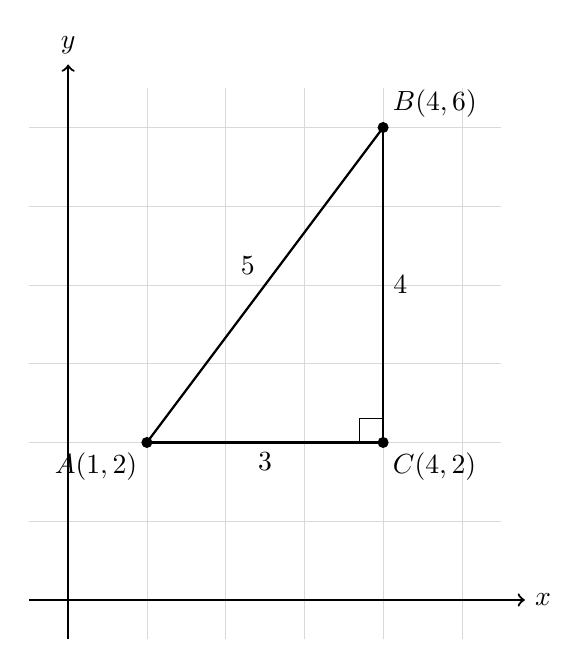
\begin{tikzpicture}[scale=1]
  \draw[step=1,gray!30,very thin] (-0.5,-0.5) grid (5.5,6.5);
  \draw[->,thick] (-0.5,0) -- (5.8,0) node[right] {$x$};
  \draw[->,thick] (0,-0.5) -- (0,6.8) node[above] {$y$};
  \fill (1,2) circle (2pt) node[below left] {$A(1,2)$};
  \fill (4,6) circle (2pt) node[above right] {$B(4,6)$};
  \fill (4,2) circle (2pt) node[below right] {$C(4,2)$};
  \draw[thick] (1,2) -- (4,2) node[midway,below] {$3$};
  \draw[thick] (4,2) -- (4,6) node[midway,right] {$4$};
  \draw[thick] (1,2) -- (4,6) node[midway,above left] {$5$};
  \draw (3.7,2) -- (3.7,2.3) -- (4,2.3);
\end{tikzpicture}
\end{center}

这个公式值得多看两眼。左边 $AB$ 是几何对象——一段线段的长度；右边是代数对象——一堆坐标的四则运算和开方。一个公式，两种语言，这就是坐标桥梁通车的第一辆车。

\begin{fanli}
“$A$ 在 $(1,2)$，$B$ 在 $(4,6)$，横向差 $3$，纵向差 $4$，所以距离是 $3+4=7$。”——错。$3+4$ 算出来的是“先水平走、再竖直走”的折线长度，像出租车沿着方格马路绕路走的里程；而两点间的距离指直线段的长度，是斜着抄近路的那一条。勾股定理告诉我们斜边是 $\sqrt{3^{2}+4^{2}}=5$，恰好比 $7$ 小，这与“两点之间线段最短”完全一致。把坐标差直接相加，是把马路里程当成了直线距离。
\end{fanli}

距离公式还有一个好用的副产品。线段 $AB$ 的中点 $M$ 该是什么坐标？直觉是“各取一半的平均”，这个直觉是对的：

\begin{tuilun}[中点公式]
点 $A(x_{1},y_{1})$ 与点 $B(x_{2},y_{2})$ 连线的中点 $M$ 的坐标为
\[
M\left(\frac{x_{1}+x_{2}}{2},\ \frac{y_{1}+y_{2}}{2}\right).
\]
\end{tuilun}

道理可以这样想：从 $A$ 走到 $B$，横坐标一共变化 $x_{2}-x_{1}$，走到一半就是变化一半，所以中点横坐标是 $x_{1}+\frac{x_{2}-x_{1}}{2}=\frac{x_{1}+x_{2}}{2}$；纵坐标同理。严格的证明可以把 $M$ 的坐标代入距离公式，验证 $AM=MB=\frac{1}{2}AB$ 即可，留给你动手。比如 $A(1,2)$、$B(4,6)$ 的中点是 $(\frac{5}{2},4)$，也就是 $(2.5,4)$，看图上的位置，确实在线段正中间。

\section{方程是形状的身份证}

到目前为止，我们是“先有图形，后算坐标”。现在把方向调过来，问一个更好玩的问题：\textbf{给平面上所有的点立一个规矩，守规矩的点会组成什么图形？}

比如这条规矩：“到原点的距离等于 $3$。”凭几何直觉，你大概已经喊出答案了：一个圆！圆的定义本来就是这样。但我们假装不知道，用坐标把这件事重新走一遍。设守规矩的点坐标是 $(x,y)$，它到原点 $(0,0)$ 的距离由距离公式给出，规矩翻译成代数语言就是：

\[
\sqrt{x^{2}+y^{2}}=3,\quad\text{两边平方得}\quad x^{2}+y^{2}=9.
\]

于是一个几何条件（到某点距离固定）变成了一个代数方程（$x^{2}+y^{2}=9$）。这个方程像一个筛子：点 $(3,0)$ 的坐标代进去，$9+0=9$，成立，它在圆上；点 $(1,2)$ 代进去，$1+4=5\ne 9$，它不在圆上；点 $(\sqrt{5},2)$ 代进去，$5+4=9$，它在圆上。平面上亿万个点，每个点要么通过筛子、要么被筛掉，而通过筛子的点连起来，正好是以原点为圆心、$3$ 为半径的圆，一个不多，一个不少。

\begin{dingyi}[曲线的方程与轨迹]
如果一个方程 $F(x,y)=0$ 与一条曲线满足两方面的对应：曲线上每个点的坐标都满足方程，坐标满足方程的每个点都在曲线上，那么这个方程叫做这条曲线的方程，这条曲线叫做这个方程的图形（轨迹）。
\end{dingyi}

“轨迹”这个词很形象：一个守规矩的点在平面上跑动，它跑过的痕迹就是轨迹。规矩用代数写出来是方程，痕迹用几何画出来是曲线。请看下面这张“对照表”：

\begin{center}
\begin{tabular}{ll}
\toprule
代数一侧：方程 & 几何一侧：图形 \\
\midrule
$y=2x-1$ & 一条直线（斜率 $2$，过点 $(0,-1)$） \\
$x^{2}+y^{2}=9$ & 以原点为圆心、$3$ 为半径的圆 \\
$y=x^{2}$ & 开口向上的抛物线，顶点在原点 \\
\bottomrule
\end{tabular}
\end{center}

直线的那一行你在第 2 章已经见过：一次函数 $y=kx+b$ 的图像是一条直线。现在你知道这件事的新说法了：二元一次方程 $y=kx+b$ 的轨迹是直线。抛物线那一行也值得亲手验证：取 $x=0,\pm1,\pm2$ 算出 $y=0,1,1,4,4$，在坐标纸上描出这五个点，用光滑的曲线连起来，就是那条著名的碗形曲线。

\begin{center}
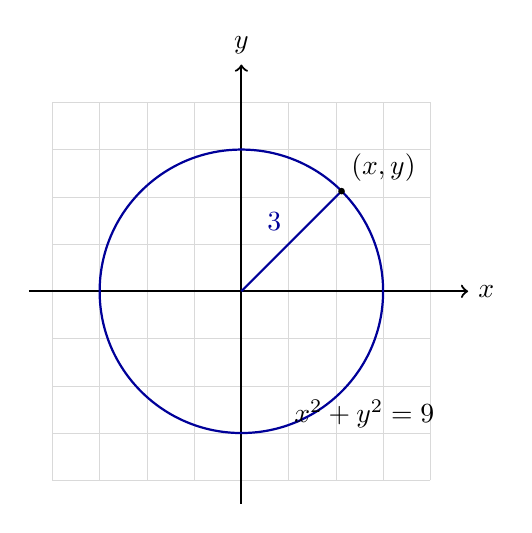
\begin{tikzpicture}[scale=0.6]
  \draw[step=1,gray!30,very thin] (-4,-4) grid (4,4);
  \draw[->,thick] (-4.5,0) -- (4.8,0) node[right] {$x$};
  \draw[->,thick] (0,-4.5) -- (0,4.8) node[above] {$y$};
  \draw[thick,blue!60!black] (0,0) circle (3);
  \draw[thick,blue!60!black] (0,0) -- (2.12,2.12) node[midway,above left] {$3$};
  \fill (2.12,2.12) circle (2pt) node[above right] {$(x,y)$};
  \node at (2.6,-2.6) {$x^{2}+y^{2}=9$};
\end{tikzpicture}
\hspace{8mm}
\begin{tikzpicture}[scale=0.6]
  \draw[step=1,gray!30,very thin] (-4,-1) grid (4,5);
  \draw[->,thick] (-4.5,0) -- (4.8,0) node[right] {$x$};
  \draw[->,thick] (0,-1.2) -- (0,5.5) node[above] {$y$};
  \draw[thick,blue!60!black,domain=-2.2:2.2,smooth] plot (\x,{0.5*\x*\x});
  \fill (0,0) circle (2pt) node[below right] {$(0,0)$};
  \fill (2,2) circle (2pt) node[below right] {$(2,2)$};
  \fill (-2,2) circle (2pt) node[below left] {$(-2,2)$};
  \node at (2.8,4.6) {$y=x^{2}$（纵向压缩画出）};
\end{tikzpicture}
\end{center}

\begin{li}
判断点 $P(2,\sqrt{5})$ 是否在圆 $x^{2}+y^{2}=9$ 上，并说明它在圆内还是圆外。

把坐标代入方程左边：$2^{2}+(\sqrt{5})^{2}=4+5=9$，恰好等于右边，所以 $P$ 在圆上。再看点 $Q(1,1)$：$1^{2}+1^{2}=2<9$，它到原点的距离是 $\sqrt{2}$，小于半径 $3$，所以在圆内。一般地，$x^{2}+y^{2}<9$ 的点在圆内，大于 $9$ 的在圆外——一个等式分出曲线，两个不等式分出曲线的两侧，全是距离公式在背后工作。
\end{li}

\begin{shiyan}
拿一张坐标纸（或自己画格子的白纸），标出两个点 $A(0,0)$ 和 $B(4,0)$。现在寻找“到 $A$、$B$ 距离相等”的点：先用尺子量着找，比如 $(2,0)$ 显然算一个；$(2,1)$ 到两点的距离都是 $\sqrt{5}$，也算；$(2,3)$、$(2,-2)$ 呢？多描几个这样的点，看看它们排成了什么——一条竖直的直线，正是线段 $AB$ 的垂直平分线。再用代数验证一遍：设 $(x,y)$ 到 $A$、$B$ 距离相等，则 $\sqrt{x^{2}+y^{2}}=\sqrt{(x-4)^{2}+y^{2}}$，两边平方化简，$x^{2}=(x-4)^{2}$，展开得 $8x=16$，即 $x=2$。几何里需要作图才能找到的垂直平分线，代数里化简两行就出现了。
\end{shiyan}

\section{翻译演示之一：用代数做几何题}

桥是双向的，我们先走“几何到代数”这个方向。选一道经典的几何题：

\textbf{题目（三角形中位线定理）}：连接三角形两边中点的线段，平行于第三边，并且长度等于第三边的一半。

第 3 章里，这类题的标准打法是作辅助线、凑全等三角形——需要一点灵感，而灵感这东西不是每次都准时到场。坐标法提供的则是另一种性格的路线：不需要灵感，只需要耐心。我们把这个定理用坐标完整证一遍。

设三角形的三个顶点为 $A(x_{1},y_{1})$、$B(x_{2},y_{2})$、$C(x_{3},y_{3})$。注意这里故意不用具体数字，因为定理对\textbf{所有}三角形成立，字母正好代表“任意”。

第一步，翻译已知。设 $M$ 是 $AB$ 的中点，$N$ 是 $AC$ 的中点。由中点公式：

\[
M\left(\frac{x_{1}+x_{2}}{2},\frac{y_{1}+y_{2}}{2}\right),\qquad
N\left(\frac{x_{1}+x_{3}}{2},\frac{y_{1}+y_{3}}{2}\right).
\]

第二步，翻译结论之“一半”。用距离公式算 $MN$。横坐标之差为

\[
\frac{x_{1}+x_{3}}{2}-\frac{x_{1}+x_{2}}{2}=\frac{x_{3}-x_{2}}{2},
\]

纵坐标之差同理为 $\frac{y_{3}-y_{2}}{2}$。于是

\[
MN=\sqrt{\left(\frac{x_{3}-x_{2}}{2}\right)^{2}+\left(\frac{y_{3}-y_{2}}{2}\right)^{2}}
=\frac{1}{2}\sqrt{(x_{3}-x_{2})^{2}+(y_{3}-y_{2})^{2}}=\frac{1}{2}\,BC.
\]

“长度等于第三边的一半”证完了。注意每一步都只是通分、提公因数 $\frac{1}{2}$、套距离公式，没有任何一步需要灵感。

第三步，翻译结论之“平行”。两条线段平行，在坐标里是什么意思？看方向：从 $M$ 到 $N$，横坐标变化 $\frac{x_{3}-x_{2}}{2}$，纵坐标变化 $\frac{y_{3}-y_{2}}{2}$；从 $B$ 到 $C$，横坐标变化 $x_{3}-x_{2}$，纵坐标变化 $y_{3}-y_{2}$。前者的每一个变化量恰好都是后者的一半——两段路“横纵步伐的比例”完全一样，所以方向相同，$MN$ 与 $BC$ 平行。（如果 $x_{3}=x_{2}$，则两个横坐标变化都是 $0$，两条线段都是竖直的，依然平行。）定理证毕。

回头品味一下这种解法。几何证法像一位侦探，要灵光一闪找到那条辅助线；坐标证法像一台碾米机，把图形碾成坐标，把结论碾成等式，然后按部就班地碾下去，出口处就是证明。碾米机不浪漫，但它从不旷工。而且坐标法有一个几何法比不了的好处：\textbf{它能批量处理}。同样的套路，换成“三条中线交于一点”“对角线互相平分”等一大批定理，几乎原样照搬，全都碾得出来。这正是代数“一次解决一整类问题”的精神，借坐标桥开进了几何的地盘。

\section{翻译演示之二：用几何解代数题}

反方向的车也发一班。看一道让代数方法皱眉头的题：

\textbf{题目}：当 $x$ 取什么值时，式子
\[
f(x)=\sqrt{x^{2}+9}+\sqrt{(6-x)^{2}+16}
\]
取得最小值？最小值是多少？

纯代数地看，这题相当棘手：两个根号套着平方，配方配不干净，平方又越弄越复杂。初中生手里的代数工具对它基本无效。但如果你刚走完上一节，应该会冒出一个念头：这两个根号，长得太像距离公式了。

$\sqrt{x^{2}+9}=\sqrt{(x-0)^{2}+(0-3)^{2}}$，这是点 $(x,0)$ 到点 $(0,3)$ 的距离。$\sqrt{(6-x)^{2}+16}=\sqrt{(x-6)^{2}+(0-(-4))^{2}}$，这是点 $(x,0)$ 到点 $(6,-4)$ 的距离。于是整个式子在说：在 $x$ 轴上取一点 $P(x,0)$，它到 $A(0,3)$ 和 $B(6,-4)$ 的距离之和是 $PA+PB$。题目变成了——

\textbf{翻译后的几何题}：$x$ 轴上有一动点 $P$，$A$ 在轴上方，$B$ 在轴下方，求 $PA+PB$ 的最小值。

这道题几何上几乎是白给的：两点之间，线段最短。$A$、$B$ 分居 $x$ 轴两侧，连接 $A$、$B$ 的线段必然穿过 $x$ 轴，交点就是我们找的 $P$。此时 $PA+PB$ 正好等于 $AB$；$P$ 挪到任何别的位置，$PA+PB$ 都是一条折线，必然更长。所以最小值就是

\[
AB=\sqrt{(6-0)^{2}+(-4-3)^{2}}=\sqrt{36+49}=\sqrt{85}.
\]

$\sqrt{85}$ 约等于 $9.22$。如果想把 $x$ 也求出来：直线 $AB$ 从 $(0,3)$ 走到 $(6,-4)$，横向每走 $6$ 格、纵向下降 $7$ 格，走到 $x$ 轴上意味着纵坐标从 $3$ 降到 $0$，占总下降量的 $\frac{3}{7}$，所以横向也走了总量的 $\frac{3}{7}$，$x=6\times\frac{3}{7}=\frac{18}{7}$。你可以把 $x=\frac{18}{7}$ 代回原来的式子验算，两个根号加起来正好是 $\sqrt{85}$。

请停下来感受一下刚才发生了什么。我们\textbf{没有把那个代数式算出来}——我们只是认出它的几何化身，然后引用了一条三岁小孩都能理解的原理：直线比折线短。代数里面目狰狞的最小值问题，几何里是一个一目了然的事实。这就是翻译的第二种用法：当一种语言里说不清楚时，换到另一种语言里，难题可能自己会亮出底牌。

\begin{lianjie}
这种“翻译”不是书斋里的游戏。导航软件每时每刻都在做本章的演示：卫星告诉它你的经纬度（坐标），它把街道变成平面上的线，把“怎么走最近”变成距离与折线的问题。电脑游戏里的角色沿着抛物线跳跃，那是程序在反复计算 $y=x^{2}$ 一类的方程；医生看的 CT 图像，本质是机器把人体切面上每个点的“密度数对”重建成了图形。往后看，第 2 章的函数图像是“方程变曲线”的第一次亮相，本章把它变成了系统的方法；第 7 章的向量会让“点的平移和旋转”也能代数化；而微积分里最核心的动作——研究曲线的弯曲与变化——每一步都踩在这座坐标桥上。
\end{lianjie}

\section{让点动起来：参数方程}

到目前为止，方程描述的都是静态的画面：哪些点在曲线上，哪些不在。但现实世界里的点几乎都在动：秒针尖端绕着表盘转，抛出去的篮球划出弧线，游戏角色在屏幕上奔跑。怎么给“运动”本身写一个方程？

再看一眼我们的老朋友，抛物线 $y=x^{2}$。换一种眼光：把它想象成一个小球爬出来的痕迹。设小球从原点出发，向右爬的速度是每秒 $1$ 个单位，而它的高度按规则随时间变化——用 $t$ 表示出发后的秒数，那么

\[
x=t,\qquad y=t^{2}.
\]

$t=0$ 时小球在 $(0,0)$；$t=1$ 时在 $(1,1)$；$t=2$ 时在 $(2,4)$；$t=3$ 时在 $(3,9)$。每一秒，小球都有一个确定的位置，所有位置连起来，还是那条抛物线。看出区别了吗？$y=x^{2}$ 说的是“横纵坐标之间的关系”，不管点什么时候到；而 $x=t$、$y=t^{2}$ 这一对方程说的是“每个时刻点在哪里”——它不仅画出了轨迹，还记录了行程表。这个多出来的变量 $t$ 叫做\textbf{参数}，这样的一对方程叫做\textbf{参数方程}。

\begin{dingyi}[参数方程]
如果曲线上动点的坐标 $(x,y)$ 分别表示成某个变量 $t$ 的式子
\[
x=f(t),\qquad y=g(t),
\]
当 $t$ 取遍允许的值时，$(x,y)$ 正好描出这条曲线，那么这对方程叫做曲线的参数方程，$t$ 叫做参数。
\end{dingyi}

参数常常扮演“时间”的角色，但它不是非得是时间不可，它只是一个“指挥棒”：$t$ 变，点就走。来一个更像物理的例子。把一个小球水平抛出，忽略空气阻力，它向右匀速、向下加速（这里简化数字，不追求精确的重力数据）：

\[
x=2t,\qquad y=5-t^{2}\quad(t\ge 0).
\]

$t=0$ 时球在 $(0,5)$，出手高度 $5$；$t=1$ 时在 $(2,4)$；$t=2$ 时在 $(4,1)$；$t$ 再大一点，$y$ 变负，球落地了。如果我只关心球划出的弧线形状、不关心时刻，可以把参数\textbf{消掉}：由第一式得 $t=\frac{x}{2}$，代入第二式：

\[
y=5-\left(\frac{x}{2}\right)^{2}=5-\frac{x^{2}}{4}.
\]

参数不见了，剩下一条开口向下的抛物线——平抛运动的轨迹果然是抛物线，和投篮、喷泉的水柱是同一个家族。从参数方程消去 $t$，就回到普通方程；反过来，同一条曲线可以有许多不同的参数方程，对应“以不同方式走这条路”：$x=t$、$y=t^{2}$ 是匀速横移地爬抛物线，$x=t^{3}$、$y=t^{6}$ 描出的是同一段弧的右半边，只是节奏不同。轨迹是舞台，参数方程是剧本——舞台只有一个，剧本可以写很多本。

为什么非要让点动起来？因为太多的问题天然带着“时间”或者“进度”：行星什么时候走到离太阳最近，炮弹落在哪里，动画里这一帧角色该画在屏幕哪个像素。静态方程回答“在哪条路上”，参数方程回答“此刻在路上的哪一点”。后者显然更接近工程师和物理学家真正想问的东西。

\begin{pandeng}
坐标桥的另一端通向一片很大的大陆，关键词包括：\textbf{解析几何}——系统研究“方程与曲线互译”的学科，笛卡尔和费马被公认为它的两位奠基人，据说两人还为此争执过优先权；\textbf{圆锥曲线}——椭圆、抛物线、双曲线为什么都叫“圆锥”曲线，它们和行星轨道有什么关系；\textbf{极坐标}——用“距离加方向”而不只“横纵”来给点编地址，雷达屏幕用的就是它；\textbf{参数方程与微积分}——知道行程表 $x=f(t)$、$y=g(t)$，怎样求每一刻的速度。这些名词现在不懂完全没有关系，把它们当作地图上尚未解锁的区域即可。
\end{pandeng}

\begin{toolbox}
本章新增的工具，按出场顺序：

\begin{itemize}
\item \textbf{数轴与一一对应}：实数与数轴上的点一一对应；一维距离 $=\lvert b-a\rvert$。
\item \textbf{平面直角坐标系}：平面上的点与有序数对 $(x,y)$ 一一对应，顺序不可乱。
\item \textbf{距离公式}：$AB=\sqrt{(x_{2}-x_{1})^{2}+(y_{2}-y_{1})^{2}}$，本质是坐标化的勾股定理。
\item \textbf{中点公式}：中点坐标是两端坐标的平均。
\item \textbf{方程与轨迹互译}：点在曲线上，当且仅当它的坐标满足曲线的方程；几何条件可以筛出一个方程，一个方程可以描出一条曲线。
\item \textbf{双向解题}：几何题可以设坐标“硬算”，代数题（尤其含根号的）可以翻译成距离“巧看”。
\item \textbf{参数方程}：用第三个变量 $t$ 记录动点的行程表；消去参数回到普通方程。
\end{itemize}
\end{toolbox}

\section*{思考题}

\textbf{观察题}

\begin{sikao}
\item 取 $t=-2,-1,0,1,2$，分别计算参数方程 $x=t^{2}$、$y=2t$ 给出的点，描在坐标纸上连成光滑曲线。它像什么形状？提示：由第二式解出 $t=\frac{y}{2}$，代入第一式消去 $t$，看看 $x$ 和 $y$ 满足什么方程——它和 $y=x^{2}$ 是什么关系？
\item 在坐标纸上把满足 $x^{2}+y^{2}\le 9$ 的点所在区域涂上阴影，再把满足 $x+y>0$ 的区域用另一种方式标出。两块重叠的部分像什么？提示：先分别画出两条边界 $x^{2}+y^{2}=9$ 和 $x+y=0$，不等式对应边界的哪一侧，可以代一个试点（比如原点）来判断。
\end{sikao}

\textbf{证明题}

\begin{sikao}
\item 用坐标证明：对角线互相平分的四边形是平行四边形。提示：把两条对角线的公共中点设在原点，两个对角顶点设为 $(a,b)$ 与 $(-a,-b)$，另两个设为 $(c,d)$ 与 $(-c,-d)$，再比较两组对边的“横纵步伐”。
\item 平面上两定点 $A(-1,0)$、$B(1,0)$，动点 $P(x,y)$ 满足 $PA^{2}+PB^{2}=10$。证明 $P$ 的轨迹是一个圆，并指出圆心和半径。提示：把 $PA^{2}$、$PB^{2}$ 用距离公式展开（注意是距离的\textbf{平方}，根号正好消失），合并同类项后观察。
\end{sikao}

\textbf{挑战题}

\begin{sikao}
\item 求 $\sqrt{x^{2}-2x+2}+\sqrt{x^{2}-8x+20}$ 的最小值。提示：先把每个根号里配方，认出两个“距离”；这次两个定点在 $x$ 轴的同一侧，直接连线不管用——想想照镜子：把其中一个点关于 $x$ 轴对称过去，折线长度不变，直线就可以登场了。
\item 动点 $P$ 沿抛物线 $y=x^{2}$ 移动，坐标可写为 $(t,t^{2})$；定点 $A$ 为 $(2,0)$。写出 $PA^{2}$ 关于 $t$ 的表达式。提示：用距离公式后不要急着开方——$PA^{2}$ 会是一个关于 $t$ 的\textbf{四次}式子。它有没有最小值、在什么时候取得，靠初中配方已经看不出来了；这个“看不懂的四次式”正是下一章要对付的东西。
\end{sikao}

\section*{通往下一章的门}

这座桥通车之后，最先被运过河的货物，是我们本章见过好几次的那条曲线——抛物线。

把抛物线 $y=x^{2}-3x+2$ 画在坐标纸上，你会发现它和 $x$ 轴碰了两次面。碰撞点的纵坐标是 $0$，所以横坐标必须满足 $x^{2}-3x+2=0$——一个二次方程。这就是说，\textbf{曲线与 $x$ 轴的交点，和方程的根，是同一件东西的两种说法}：一个在几何里用眼睛看，一个在代数里用计算求。方程 $x^{2}-3x+2=0$ 有根 $1$ 和 $2$，抛物线就正好在 $(1,0)$ 和 $(2,0)$ 两处碰到 $x$ 轴。

于是一连串新问题顺着桥面涌了过来。把 $2$ 次换成 $3$ 次，$y=x^{3}-x$ 这条曲线会和 $x$ 轴碰几次？换成 $4$ 次、$5$ 次呢？有没有一条多项式曲线，永远不碰 $x$ 轴——也就是说，有没有一个方程根本没有实数根？如果方程没有实数根，是“题目出错了”，还是“数的世界太小了，该扩建了”？

这些问题的共同主角，是 $x^{2}-3x+2$、$x^{3}-x$ 这类由字母的幂加加减减拼起来的式子——\textbf{多项式}。它们看上去只是代数的零件，却藏着方程的根、曲线的交点、甚至新数系诞生的线索。下一站，我们就把多项式拆开，看看里面的结构。
